\documentclass[aip,jcp,amsmath,amssymb,preprint,floatfix]{revtex4-1}
\usepackage[utf8]{inputenc}
\usepackage{graphicx,bm,booktabs,mathtools}
\usepackage{xcolor}
\usepackage[version=4]{mhchem}
\usepackage{hyperref}
\hypersetup{hidelinks}
\setlength{\emergencystretch}{1em}
\newcommand{\Tr}{\operatorname{Tr}}
\newcommand{\spec}{\operatorname{spec}}
\newcommand{\supp}{\operatorname{supp}}
\newcommand{\ran}{\operatorname{ran}}
\newcommand{\dd}{\mathrm{d}}
\newcommand{\Eh}{E_{\mathrm h}}
\newcommand{\au}{\mathrm{a.u.}}
\newcommand{\Heff}{\hat{H}_{\mathrm{eff}}}
\newcommand{\G}{\mathcal G}
\newcommand{\D}{\mathcal D}
\newcommand{\Rop}{\hat{\mathcal R}_Q}

% Hats mark operators; explicit matrices, matrix elements, and scalars are unhatted.

\renewcommand{\thesection}{S\arabic{section}}
\renewcommand{\thesubsection}{\thesection.\arabic{subsection}}
\renewcommand{\theequation}{S\arabic{equation}}
\renewcommand{\thefigure}{S\arabic{figure}}
\renewcommand{\thetable}{S\arabic{table}}
\begin{document}
\title{Supplementary Material: Multistate Quantum Geometry Distinguishes Physical Response from Electronic-State Switching}
\author{Hui Li}\author{Dongbo Zhao}
\email{dongbo@ynu.edu.cn}
\affiliation{Institute of Biomedical Research, School of Life Sciences, Yunnan University, Kunming 650500, China}
\date{22 October 2026}\maketitle

\noindent
This Supplementary Material provides the derivations, numerical criteria, and
data definitions used in the main text. Sections S1--S5 concern the theory;
Sec.~S6 documents the molecular calculations; Sec.~S7 describes independent
checks of the equations and archived tables. Data and scripts are available in the
\href{https://github.com/zzdbl520/quantum-geometry-response-data/tree/main/multistate}{public reproducibility repository}.
Its README identifies the files used for each result.

\section{Resolvent expansion and its domain}
At fixed nuclear geometry, let $\hat H(F)=\hat H_0-F\hat\mu$.
The spectral projector $\hat P$ selects the electronic states of interest,
and $\hat Q=\hat I-\hat P$ selects their complement. We use
$\hat H_P=\hat P\hat H_0\hat P$, $\hat H_Q=\hat Q\hat H_0\hat Q$,
$\hat\mu_P=\hat P\hat\mu\hat P$, $\hat\mu_Q=\hat Q\hat\mu\hat Q$,
and $\hat B=\hat Q\hat\mu\hat P$. The resolvent is
$\Rop(E)=(\hat H_Q-E\hat Q)^{-1}$ on the complementary space.
Unless specified otherwise, its energy argument is suppressed below.
Hats denote operators; explicit matrices, matrix elements, and scalar quantities are unhatted, as in the main text. All inverses in this section are restricted to $\operatorname{ran}\hat{Q}$, not the full space. Starting from
\begin{equation}
(\hat{H}_Q-E\hat{Q}-F\hat{\mu}_Q)q=F\hat{B}p,
\end{equation}
write the inverse as
\begin{equation}
(\hat{H}_Q-E\hat{Q}-F\hat{\mu}_Q)^{-1}
=(\hat{I}-F\Rop\hat{\mu}_Q)^{-1}\Rop
=\Rop+F\Rop\hat{\mu}_Q\Rop+O(F^2).
\end{equation}
The Neumann expansion is sufficient when $|F|\|\Rop\hat{\mu}_Q\|<1$. Substitution into the $\hat{P}$ equation gives
\begin{equation}
\Heff(E,F)=\hat{H}_P-F\hat{\mu}_P-F^2\hat{B}^\dagger\Rop \hat{B}
-F^3\hat{B}^\dagger\Rop\hat{\mu}_Q\Rop \hat{B}+O(F^4).
\end{equation}
The projected Schr{\"o}dinger equation therefore gives the second-order response matrix.\cite{Lowdin1951,Feshbach1962} If $E(F)=E_\star+O(F)$, expanding $\Rop(E(F))$ changes the quadratic term only at order $F^3$. At a true pole of the resolvent the expansion is invalid. Applying a pseudoinverse to $\hat{M}_2$ cannot restore it.

The one-state expression follows by setting $\hat{P}=|0\rangle\langle0|$ and expanding the complementary resolvent in eigenstates. For an excited state, signed denominators are retained. Positivity of the metric does not imply positivity of the polarizability.

\section{Uncoupled state combinations and the response factorization}
Put $\hat{T}=\Rop \hat{B}$, so $\hat{M}_2=\hat{T}^\dagger \hat{T}$. Then
\begin{equation}
\langle v|\hat{M}_2|v\rangle=\|\hat{T}|v\rangle\|^2,\qquad
\ker \hat{M}_2=\ker \hat{T}=\ker \hat{B}.
\end{equation}
If $|v\rangle$ lies in this kernel, $\hat{M}_1|v\rangle=\hat{B}^\dagger\Rop \hat{B}|v\rangle=0$. Hermiticity then gives both $\hat{M}_1(\hat{I}-\hat{\Pi})=0$ and $(\hat{I}-\hat{\Pi})\hat{M}_1=0$, where $\hat{\Pi}$ projects onto $\ran \hat{M}_2$. Thus $\hat{\Pi} \hat{M}_1\hat{\Pi}=\hat{M}_1$, even if $\hat{M}_1$ has additional null vectors from positive/negative-denominator cancellation.

For a Hermitian positive-semidefinite operator, diagonalization constructs its Moore--Penrose inverse,\cite{Penrose1955}
\begin{equation}
\hat{M}_2^+=\sum_{\lambda_a>0}\lambda_a^{-1}|a\rangle\langle a|.
\end{equation}
It satisfies the four defining relations
\begin{align}
\hat{M}_2\hat{M}_2^+\hat{M}_2&=\hat{M}_2,&\hat{M}_2^+\hat{M}_2\hat{M}_2^+&=\hat{M}_2^+,\\
(\hat{M}_2\hat{M}_2^+)^\dagger&=\hat{M}_2\hat{M}_2^+,&
(\hat{M}_2^+\hat{M}_2)^\dagger&=\hat{M}_2^+\hat{M}_2.
\end{align}
The square root $\hat{W}=(\hat{M}_2^+)^{1/2}$ therefore inverts only directions with nonzero external dipole coupling. Direct multiplication gives
\begin{equation}
\hat{M}_2^{1/2}(\hat{W}\hat{M}_1\hat{W})\hat{M}_2^{1/2}=\hat{\Pi} \hat{M}_1\hat{\Pi}=\hat{M}_1.
\end{equation}
No commutation between the two moments has been used.

If $\hat{\mathcal D}|y\rangle=\delta|y\rangle$ on the support, setting $|v\rangle=\hat{W}|y\rangle$ gives $\hat{M}_1|v\rangle=\delta\hat{M}_2|v\rangle$. Conversely, $|y\rangle=\hat{M}_2^{1/2}|v\rangle$ maps the supported generalized problem back to $\hat{\mathcal D}$. Null-space zeros added by representing $\hat{\mathcal D}$ in the full retained space are not extra physical response channels. Expanding the generalized Rayleigh quotient in external eigenstates yields the positive weights in the main-text weighted-gap expression; signed effective gaps can cancel.

Writing the operators as matrices in the chosen frames, a retained-frame rotation $U$ gives $B\mapsto BU$, $M_k\mapsto U^\dagger M_kU$. Spectral functional calculus gives $W\mapsto U^\dagger WU$, hence $\D\mapsto U^\dagger\D U$. Traces, eigenvalues, and the generalized spectrum are invariant. This statement is distinct from invariance of individual matrix entries.

In numerical work a threshold defines the supported range. The reaction analysis code uses $\lambda>\max(10^{-10}\lambda_{\max},10^{-14})$ in its working units. Thresholding is an additional approximation. For any independently obtained pair $(A,\G)$, one must test
\begin{equation}
r_{\rm supp}=\frac{\|A-\Pi A\Pi\|_F}{\max(\|A\|_F,\epsilon)}
\end{equation}
before claiming a full congruence. A negative metric eigenvalue larger than the numerical error should be investigated, not silently projected away. The reaction results do not establish convergence of the full response matrix or its response-weighted energy spectrum.

\section{Projector derivative, canonical effective Hamiltonian, and finite width}
Differentiating $\hat{P}^2=\hat{P}$ and multiplying by $\hat{P}$ and $\hat{Q}$ gives
\begin{equation}
\hat{P}(\partial_F\hat{P})\hat{P}=0,\qquad \hat{Q}(\partial_F\hat{P})\hat{Q}=0.
\end{equation}
Since $\hat{P}$ is Hermitian, $\partial_F\hat{P}=\hat{X}+\hat{X}^\dagger$, with $\hat{X}=\hat{Q}(\partial_F\hat{P})\hat{P}$. Consequently
\begin{equation}
\tfrac12\Tr[(\partial_F\hat{P})^2]=\Tr(\hat{X}^\dagger \hat{X}).
\end{equation}
Differentiating $[\hat{H},\hat{P}]=0$ for $\hat{H}'=-\hat{\mu}$ gives
\begin{equation}
[\hat{H}_0,\partial_F\hat{P}]=[\hat{\mu},\hat{P}].
\end{equation}
Its $\hat{Q}\hat{P}$ block is $\hat{H}_Q\hat{X}-\hat{X}\hat{H}_P=\hat{B}$. For Hermitian blocks, diagonalization turns this into $(E_n-E_a)X_{na}=B_{na}$. This proves uniqueness for disjoint spectra and directly establishes the external-gap bound in the main text. It also explains the Sylvester equation without assuming familiarity with a matrix-equation solver.\cite{Kato1995,BartelsStewart1972}

To derive the canonical second-order Hamiltonian, introduce the anti-Hermitian first-order generator
\begin{equation}
\hat{S}=\begin{pmatrix}0&-\hat{X}^\dagger\\\hat{X}&0\end{pmatrix},
\qquad \hat{H}_{\rm can}(F)=\hat{P} e^{-F\hat{S}}\hat{H}(F)e^{F\hat{S}}\hat{P}+O(F^3).
\end{equation}
A higher-order off-diagonal generator can cancel remaining off-diagonal terms, but does not affect the displayed diagonal block through second order. The Baker--Campbell--Hausdorff expansion is
\begin{equation}
e^{-F\hat{S}}\hat{H}(F)e^{F\hat{S}}
=\hat{H}_0+F(-\hat{\mu}+[\hat{H}_0,\hat{S}])
+F^2\left([-\hat{\mu},\hat{S}]+\tfrac12[[\hat{H}_0,\hat{S}],\hat{S}]\right)+O(F^3).
\end{equation}
The Sylvester equation cancels the first-order off-diagonal block. In the $\hat{P}\hat{P}$ block,
\begin{equation}
[-\hat{\mu},\hat{S}]_{PP}=-(\hat{B}^\dagger \hat{X}+\hat{X}^\dagger \hat{B}),\quad
[[\hat{H}_0,\hat{S}],\hat{S}]_{PP}=\hat{B}^\dagger \hat{X}+\hat{X}^\dagger \hat{B}.
\end{equation}
Thus
\begin{equation}
\hat{H}_{\rm can}(F)=\hat{H}_P-F\hat{\mu}_P-\tfrac12F^2(\hat{B}^\dagger \hat{X}+\hat{X}^\dagger \hat{B})+O(F^3).
\end{equation}
The canonical alignment has no first-order rotation internal to $\hat{P}$ and agrees to the relevant order with direct polar alignment. This construction is a form of the established unitary effective-Hamiltonian transformation.\cite{Bravyi2011}

For a finite-width cluster, let $\hat{H}_P=E_\star \hat{P}+\hat{D}_P$, $w=\|\hat{D}_P\|_2$, and $d=\operatorname{dist}(E_\star,\spec \hat{H}_Q)$. With $\hat{Y}=\Rop(E_\star)\hat{B}$,
\begin{equation}
\hat{X}=\hat{Y}+\Rop(E_\star)\hat{X}\hat{D}_P .
\end{equation}
If $\eta=w/d<1$, Frobenius-norm bounds give
\begin{equation}
\|\hat{X}\|_F\le\frac{\|\hat{Y}\|_F}{1-\eta},\qquad
\|\hat{X}-\hat{Y}\|_F\le\frac{\eta}{1-\eta}\|\hat{Y}\|_F.
\end{equation}
The metric error obeys
\begin{equation}
\|\hat{X}^\dagger \hat{X}-\hat{Y}^\dagger \hat{Y}\|_F
\le(\|\hat{X}\|_F+\|\hat{Y}\|_F)\|\hat{X}-\hat{Y}\|_F.
\end{equation}
This provides a sufficient small-width condition; no common-reference approximation is required when the Sylvester equation is solved directly.

The matrix elements $\G_{ab}=\langle a|\hat{\mathcal G}|b\rangle$ contain products of distinct denominators,
\begin{equation}
\G_{ab}=\sum_n\frac{B_{na}^*B_{nb}}{(E_n-E_a)(E_n-E_b)}.
\end{equation}
An arithmetic average of the two squared denominators is not this off-diagonal matrix, although its diagonal entries agree. Some supplied exploratory six-state code computes that alternative diagnostic. The molecular metric traces reported in the main text come from overlap estimators, and no eigenvalue of that exploratory matrix is used as an exact projector-metric result.

Support equality also fails in general. In explicit matrix form, take $H_P=\operatorname{diag}(0,0.2)$, $H_Q=1$, $X=(1,1)$ and $B=(1,0.8)$. They satisfy the Sylvester equation, but
\begin{equation}
\G=\begin{pmatrix}1&1\\1&1\end{pmatrix},\qquad
A=\begin{pmatrix}2&1.8\\1.8&1.6\end{pmatrix}.
\end{equation}
The vector $(1,-1)^T$ lies in the null space of $\G$ but not that of $A$. Therefore the exact-degeneracy support proof cannot be transferred unconditionally to a split cluster.

\section{Finite-field overlap estimators}
Here $\G=\Psi_0^\dagger\hat{\mathcal G}\Psi_0$ is the metric matrix and $I$ is the identity matrix. For orthonormal frames $\Psi_0,\Psi_F$, $S_{0F}S_{0F}^\dagger=\Psi_0^\dagger \hat{P}(F)\Psi_0$. Differentiation twice of $\hat{P}^2=\hat{P}$ gives
\begin{equation}
\hat{P} \hat{P}''\hat{P}=-2\hat{P} \hat{P}'\hat{P}'\hat{P}=-2\hat{X}^\dagger \hat{X}.
\end{equation}
Expanding $\hat{P}(\pm F)$ and averaging cancels odd powers:
\begin{equation}
\Psi_0^\dagger[\hat{P}(F)+\hat{P}(-F)]\Psi_0
=2I-2F^2\G+O(F^4).
\end{equation}
This proves the estimator in the main text. Likewise,
\begin{equation}
m-\Tr[\hat{P}(-F)\hat{P}(F)]
=4F^2\Tr(\hat{X}^\dagger \hat{X})+O(F^4),
\end{equation}
and $\Tr[\hat{P}(-F)\hat{P}(F)]=\|\Psi_{-F}^\dagger\Psi_F\|_F^2$ proves the independent chordal expression.

For a basis change $\Psi_0\mapsto\Psi_0U_0$, $\Psi_F\mapsto\Psi_FU_F$, the overlap transforms as $S\mapsto U_0^\dagger S U_F$. Its nonsingular polar factor transforms the same way, so $\widetilde H(F)\mapsto U_0^\dagger\widetilde H(F)U_0$. The field-frame gauge cancels. Under active-space changes or lost singular values this construction does not establish continuity; it only specifies the alignment if the prerequisites hold.

Some production fits include a small constant common-frame offset,
\begin{equation}
\widetilde H(F)+\widetilde H(-F)-2H_0
=C-AF^2+O(F^4).
\end{equation}
Fitting the unscaled energy difference with an intercept avoids amplifying $C$ into $C/F^2$. A fitted offset is nevertheless a diagnostic of model or solver mismatch, does not justify fitting across a change of stationary solution. The \ce{C2} release uses an absolute offset gate of $5\times10^{-8}\,\Eh$. The \ce{B2} hybrid records explicitly retain their offsets and protocol differences.

\section{Branch reconstruction and cusp derivation}
Let $\widetilde H(F)=H_0+FD-\tfrac12F^2A+\cdots$, with a nondegenerate retained eigenvalue $E_0$. First-order perturbation of its eigenvector gives
\begin{equation}
\langle j|\partial_F0\rangle=\frac{D_{j0}}{E_0-E_j}.
\end{equation}
The quadratic energy coefficient is
\begin{equation}
E_0(F)=E_0+FD_{00}
-F^2\left[\tfrac12A_{00}+
\sum_{j>0}\frac{|D_{0j}|^2}{E_j-E_0}\right]+O(F^3).
\end{equation}
Taking minus the second derivative gives the reconstruction formula. For optimized orbitals, this is a statement about the smooth matrix family actually computed. Replacing $D$ by bare transition moments changes the model and must be stated explicitly.

At degeneracy, diagonalize the first-order perturbation instead. For the first-order perturbation $-\hat{\mu}_P$, minimization selects $d_{\max}$ at positive $F$ and $d_{\min}$ at negative $F$. Writing both slopes as a common linear term plus an absolute-value term gives $\kappa=(d_{\max}-d_{\min})/2$. If the first-order matrix is scalar, subtract that common shift and diagonalize the quadratic matrix. Higher-order nonanalyticities are not excluded by the absence of a linear cusp.

\section{Computational details and numerical checks}
All three applications use the aug-cc-pVTZ basis. The electronic models and
field strengths are summarized below. A ``pass'' in an archived file refers
to that file's stated numerical criteria; it does not establish independence
from the active space or equivalence between different orbital optimizations.

\subsection{\texorpdfstring{\ce{C2}}{C2}: geometry continuity and componentwise response}
Equal-weight SA6-CASSCF(8e,8o) provides a six-state geometry frame. In the
$D_{2h}$ subgroup, the frame contains three $A_g$ roots, one $B_{1g}$ root,
and the $B_{2u}$ and $B_{3u}$ components of $^1\Pi_u$. The response target
contains $X\,{}^1\Sigma_g^+$ and both $B\,{}^1\Delta_g$ components and has
rank three. The completed continuation contains 119 geometries between
1.00 and 3.20~\AA. Earlier planning counts in the protocol files describe
the grids before adaptive refinement; the final point and edge tables
determine the reported inventory.

The internal $X/\Delta$ crossing brackets are
1.652734375--1.652812500~\AA\ and
3.0389648438--3.0390625000~\AA. Linear interpolation gives 1.65274230 and
3.03898129~\AA. The separate $\Delta/\Pi$ crossing is bracketed by
1.500 and 1.525~\AA, with an interpolated position of 1.52412071~\AA.
It closes a gap between the rank-three target and its complement.
The joint six-state geometry frame can remain continuous at this crossing,
while spectral isolation of the rank-three target fails.

The minimum adjacent active-orbital, retained-orbital, and six-state
singular values are 0.999317, 0.996936, and 0.983280, respectively.
The smallest matched state-overlap magnitude is 0.976968, and the largest
adjacent polar-factor unitarity error is $1.55\times10^{-15}$.
The largest absolute matrix element of the dipole restricted to the
$X\oplus\Delta$ space is $2.49\times10^{-14}$ a.u., consistent with
the gerade--gerade selection rule.

Signed-field magnitudes are $5\times10^{-5}$, $10^{-4}$,
$2.5\times10^{-4}$, and $5\times10^{-4}$ a.u. The numerical criteria
include a field-to-zero target singular value of at least 0.98,
an opposite-field target singular value of at least 0.95, active- and
retained-orbital singular values of at least 0.995, an energy-parity error
of at most $5\times10^{-8}\,\Eh$, a spin-square error of at most $10^{-6}$,
and a relative fit residual or stability measure of at most 0.05.
The common-frame energy-offset limit is $5\times10^{-8}\,\Eh$.
These thresholds specify numerical acceptance within this calculation.

The final plot contains 54 accepted transverse rank-three response points.
At 1.55~\AA, this target passes its component-specific criteria while an
auxiliary six-state criterion fails. The longitudinal inventory contains
35 accepted and 17 nonaccepted axis rows. A failed longitudinal response
is omitted from the relaxed curve and from any isotropic value requiring it.

Fixed-orbital CASCI calculations at 2.90, 3.0390625, and 3.20~\AA\ test
the origin of the longitudinal continuity problem. At 3.0390625~\AA,
the minimum field-to-zero and opposite-field target singular values are
0.9999974 and 0.9999894. Recovery of continuity with fixed orbitals identifies
orbital optimization as the source of the observed failure. It does not
locate a unique orbital bifurcation. These controls are used only for
continuity analysis; their response values are not inserted into the
orbital-relaxed curves.

\subsection{\texorpdfstring{\ce{B2}}{B2}: ingredients of the three-state hybrid model}
The model retains $X\,{}^3\Sigma_g^-$ and both $A\,{}^3\Pi_u$ components.
Rank three counts spatial states at fixed triplet multiplicity. It combines
state-specific zero-field energy gaps, direct common-orbital
SA3-CASSCF(6e,8o) transition moments, and backgrounds obtained from
aligned field-optimized SA3 matrices. These ingredients do not constitute
derivatives of one demonstrated common variational Hamiltonian.

The expanded data set covers 13 geometries. It contains 234 signed-field
records, 117 field pairs, and 39 axis records. Transverse field
magnitudes are $10^{-5}$, $2.5\times10^{-5}$, and $5\times10^{-5}$ a.u.;
longitudinal magnitudes are $10^{-4}$, $2.5\times10^{-4}$, and
$5\times10^{-4}$ a.u. The older seven-geometry figure in the historical
evidence directory is superseded by the 13-geometry plot generated for
the current manuscript.

At the state-specific crossing, $R_c=1.94418546$~\AA, the direct and
aligned-derivative magnitudes are 0.19743991 and approximately 0.25133 a.u.
Their ratio ranges from 1.266 to 1.284 across the grid. Comparisons use
the same zero-field reference frame; taking magnitudes removes phase-sign
ambiguities but does not make an individual entry invariant under a
general rotation of that frame.

Combining the direct coupling with the model degeneracy gives a transverse
cusp coefficient of 0.19743991 a.u. This value belongs to the stated hybrid
model. No finite transverse polarizability or rank-one metric is assigned
at that crossing. The longitudinal quantities remain finite in the model.

Original checks include a minimum transport singular value of 0.90,
a spin-square error of at most $10^{-6}$, an opposite-sign energy
difference of at most $2\times10^{-8}\,\Eh$, and a 10\% comparison
between direct and aligned-derivative magnitudes. The measured minimum
zero-field transport singular value is 0.999973. The direct/derivative
comparison fails systematically. The hybrid analysis assigns distinct
roles to these quantities and retains the original failed comparison in
the pair table; its later acceptance flag does not mean that every
original criterion passed.

\subsection{Reaction geometries and selection of the two-state space}
The geometries are from channel 1 of the H2COMBUSTION data set.
\cite{Guan2022_hydrogen_combustion}
Increasing source index follows O + OH $\rightarrow$ \ce{O2} + H.
The O--O axis defines $x$, and the charge center defines the origin.
Removing small off-axis numerical noise moves the atoms by at most
$3.0483\times10^{-6}$~\AA. The plotted coordinate is
$\xi=i/57$, where $i$ is the source index. It is not a physical arc length.
The separate Cartesian path coordinate $s$ is zero at source index 13.

The production model uses equal-weight SA4-CASSCF(13e,9o) doublet states.
The two lowest zero-field roots define the local rank-two anchor. For each
signed field, every two-column subset of the $2\times4$ anchor-overlap
matrix is considered. Candidates are ranked lexicographically by
\begin{equation}
\left(\sigma_{\min},\ \sum_a\sigma_a^2,
-\operatorname{mean}(\text{candidate indices})\right).
\end{equation}
The subset with the largest tuple is selected. Exact residual ties retain
the first subset in lexicographic enumeration. This selection is performed
at a fixed geometry; overlap with the geometry parent is a separate check.

Response records cover indices 2--11 and 15--18. Four magnitudes,
$2.5\times10^{-4}$, $5\times10^{-4}$, $7.5\times10^{-4}$, and $10^{-3}$
a.u., give 56 pairs or 112 signed-field records. The table contains selected
candidate indices, field-to-anchor and opposite-field singular values,
aligned derivative and curvature entries, and the scalar decomposition.
The minimum field-to-anchor singular value is 0.999280. The broader
zero-field calculation covered 21 geometries; this does not imply a
21-geometry response inventory in the distributed tables.

\subsection{Reaction response, field ranges, and local maxima}
For each field pair, the reconstruction is
\begin{equation}
\alpha_0(F)=A_{00}(F)+I(F),\qquad
I(F)=\frac{2|D_{01}(F)|^2}{E_1(0)-E_0(0)}.
\end{equation}
Here $D$ is the derivative of the aligned state matrix, and $A_{00}$ is
its aligned background curvature. Orbital response contributes to this
background in the optimized CASSCF calculation; it is not identified
solely with coupling to external electronic states.

For each geometry, the total is formed at every field before computing
its median and full minimum--maximum range. A sampled maximum is locally
resolved if its lower envelope exceeds the upper envelopes of both
immediate neighbors. This criterion concerns the tested field window.
The envelopes are not statistical confidence intervals and do not locate
the exact maximum of a continuous-coordinate curve.

Full-matrix extrapolation fails the response-fit residual and stability
criteria at 12 of the 14 geometries. The global 3\% scalar range criterion
fails at index 18, with relative range 0.032426. These failures are retained
alongside the locally resolved maxima at indices 5 and 9. High subspace
overlap alone does not establish convergence of every response-matrix
entry or of a response-weighted energy spectrum.

\begin{table}[ht]
\caption{Local peak checks recomputed from the four-field records. Response
values are in atomic units. The margin is the central minimum minus the
largest neighboring maximum, evaluated before rounding.}\label{tab:peaks}
\begin{ruledtabular}\begin{tabular}{lrr}
Quantity & Index 5 & Index 9\\
Total median &27.752446&24.863863\\
Minimum &27.649231&24.772465\\
Maximum &27.797117&25.268334\\
Margin above neighbors&4.679532&0.211654\\
Sum of component medians&27.756563&24.863863
\end{tabular}\end{ruledtabular}
\end{table}

The rowwise sum holds to $7.2\times10^{-15}$ a.u. The sum of the separate
component medians need not equal the median of the total, as illustrated
by index 5. For a differentiable curve, a stationary point obeys
$\dd A_{00}/\dd\xi=-\dd I/\dd\xi$; identifying a maximum additionally
requires a derivative sign change or negative curvature. The present
discrete data establish local orderings and do not directly measure those
derivatives. SA2 and state-specific curves are separate model comparisons.

\begin{figure}[ht]
\centering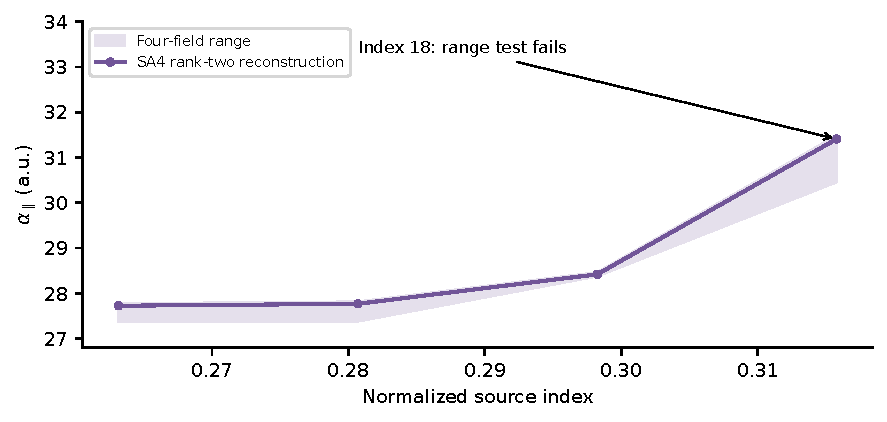
\includegraphics[width=0.9\linewidth]{../figures/HO2_controls.pdf}
\caption{Later reaction controls at indices 15--18. The envelope spans the
same four field magnitudes as the earlier peaks. Neighboring envelopes
overlap at indices 15 and 16, so these data do not resolve an additional
peak there. Index 18 fails the global 3\% field-window range criterion.}
\end{figure}

\subsection{Meaning of historical column names}
Column names are preserved to maintain correspondence with the source
files. In the reaction pair table, \texttt{dipole\_ij} stores
$[\widetilde H(+F)-\widetilde H(-F)]_{ij}/(2F)$ and therefore corresponds
to $D_{ij}$ in the main text. For a fixed-orbital Hamiltonian with
$\hat H(F)=\hat H_0-F\hat\mu$, this derivative is $-\mu_{ij}$.
The columns \texttt{alpha\_00} and
\texttt{external\_ground\_alpha\_au} both represent $A_{00}$.
The latter historical name does not remove orbital-response contributions.
The internal and reconstructed columns represent $I$ and $A_{00}+I$.
An accepted local scalar peak does not validate all other operator or
energy-scale columns contained in the same exploratory table.

\section{Independent checks of equations and numerical tables}
The two verification scripts use archived data and finite matrix models.

\texttt{scripts/verify\_revision.py} uses a fixed random seed to test
the support-restricted factorization with positive and signed gaps,
covariance under complex unitary rotations, the split-cluster Sylvester
equation, finite-field projector metrics, aligned quadratic matrices,
the support counterexample, and the three-state cusp. It also recomputes
the reaction envelopes from the individual field-pair rows.

\begin{table}[ht]
\caption{Finite-dimensional checks rerun for this release. Errors are relative
Frobenius errors unless indicated otherwise. The metric entry compares scalar
traces. Values can vary slightly with the numerical libraries.}\label{tab:verification}
\begin{ruledtabular}\begin{tabular}{lr}
Check & Error\\
Positive-gap factorization & $1.08\times10^{-15}$\\
Signed-gap factorization & $3.02\times10^{-15}$\\
Largest unitary-covariance error & $1.90\times10^{-15}$\\
Sylvester residual (absolute) & $6.52\times10^{-17}$\\
Best finite-field metric error & $1.43\times10^{-8}$\\
Best aligned quadratic-matrix error & $3.45\times10^{-8}$\\
Unsupported part of the split-cluster example & $7.83\times10^{-2}$\\

\end{tabular}\end{ruledtabular}
\end{table}


The nonzero unsupported contribution in the split-cluster counterexample
is expected: it demonstrates the need for the additional support condition.
The field-refinement table and full numerical reports are stored under
\texttt{verification/}.

\texttt{scripts/verify\_molecular\_tables.py} independently recomputes the
\ce{C2} crossings and overlap minima from the point and edge tables,
checks the \ce{B2} inventories and coupling ratios, and reconstructs
the reaction internal contribution and local peak margins. These are
checks of the distributed numerical records. They do not reconstruct
unavailable production wave functions.

\section{Data access and reproducibility scope}
The \href{https://github.com/zzdbl520/quantum-geometry-response-data/tree/main/multistate}{public reproducibility repository}
contains the molecular tables, available production and analysis scripts,
the source reaction geometries, figure-generation scripts, verification
reports, and this Supplementary Material. Its claim-to-file index identifies
which records support each main-text result. The current \ce{C2}, \ce{B2},
and reaction plots can be regenerated from the included tables without
performing new electronic-structure calculations.

The deposit preserves historical evidence files unchanged. Their older
status labels and server-specific paths describe the source calculation;
the current README and data dictionary define their use in this revision.
In particular, the older \ce{B2} seven-geometry figure is retained for
provenance and is not the current main-text figure.

Not every production checkpoint, signed-field wave function, or original
environment is present. Some original workflows require those missing
inputs. The documented reproduction commands therefore cover the
distributed-table analysis, figures, and finite-dimensional theory checks.
They do not claim a complete clean-environment rerun of all CASSCF jobs.

\bibliography{aipsamp,additional}
\end{document}

